\documentclass[border=8mm]{standalone}
\usepackage{tikz}
\usepackage{amsmath,amssymb}
\usetikzlibrary{arrows.meta, decorations.markings, calc}

\begin{document}
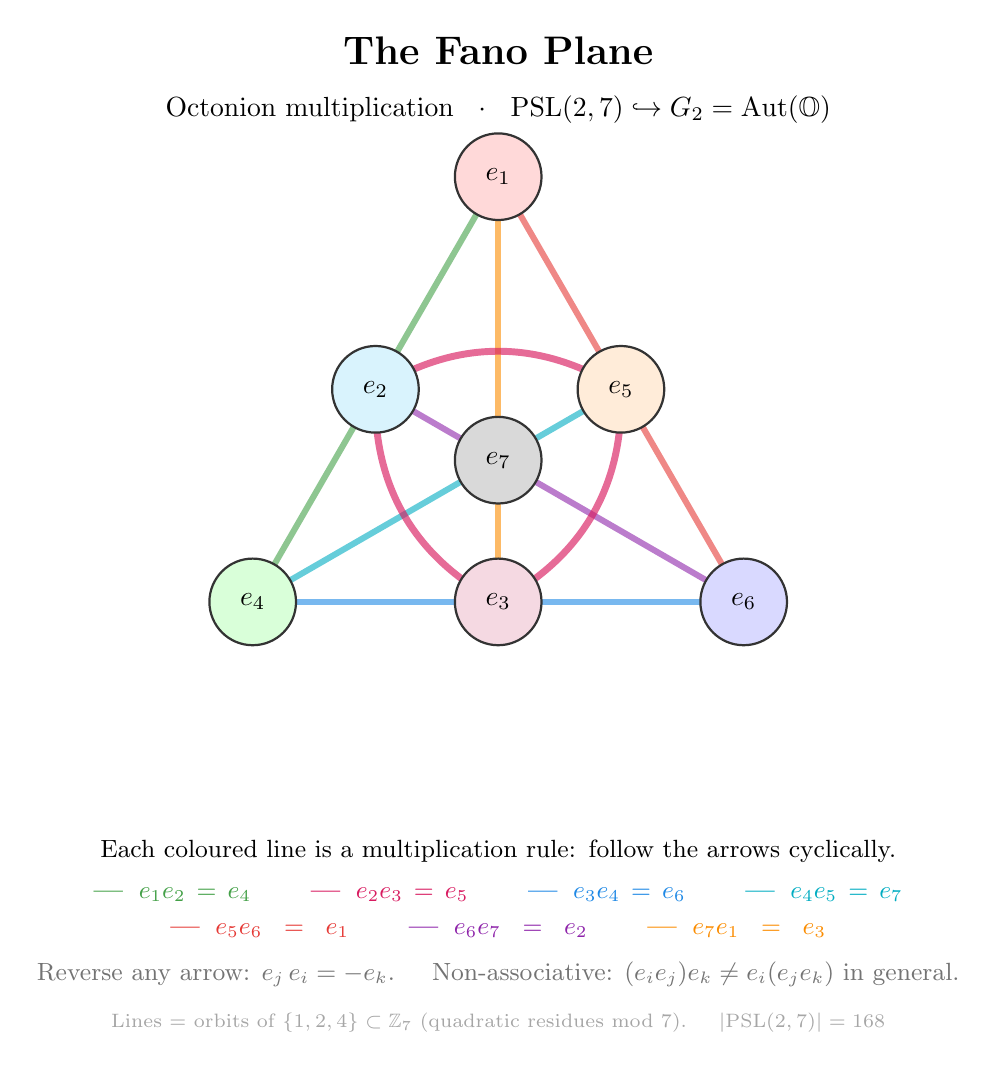
\begin{tikzpicture}[
    vtx/.style={circle, draw=black!80, fill=#1!15, minimum size=11mm,
                inner sep=0pt, font=\normalsize\bfseries, line width=0.8pt},
    vtx/.default={black},
]

% === Positions ===
% Outer triangle: e1 (top), e6 (bottom-right), e4 (bottom-left)
% Midpoints: e5 (mid 1-6), e3 (mid 4-6), e2 (mid 1-4)
% Center: e7
\def\S{3.6}
\coordinate (P1) at (90:\S);
\coordinate (P6) at (330:\S);
\coordinate (P4) at (210:\S);
\coordinate (P5) at ($(P1)!0.5!(P6)$);
\coordinate (P3) at ($(P4)!0.5!(P6)$);
\coordinate (P2) at ($(P1)!0.5!(P4)$);
\coordinate (P7) at (barycentric cs:P1=1,P4=1,P6=1);

% === Colors ===
\definecolor{cA}{HTML}{E53935}  % red — sides
\definecolor{cB}{HTML}{1E88E5}  % blue — sides
\definecolor{cC}{HTML}{43A047}  % green — sides
\definecolor{cD}{HTML}{FB8C00}  % orange — medians
\definecolor{cE}{HTML}{8E24AA}  % purple — medians
\definecolor{cF}{HTML}{00ACC1}  % cyan — medians
\definecolor{cG}{HTML}{D81B60}  % pink — circle

% === Draw 7 lines ===

% Side 1: {5,6,1} = e1—e5—e6 (right side)
\draw[cA, line width=2.2pt, opacity=0.6] (P1) -- (P6);

% Side 2: {3,4,6} = e4—e3—e6 (bottom side)
\draw[cB, line width=2.2pt, opacity=0.6] (P4) -- (P6);

% Side 3: {1,2,4} = e1—e2—e4 (left side)
\draw[cC, line width=2.2pt, opacity=0.6] (P1) -- (P4);

% Median 1: {7,1,3} = e1 through e7 to e3
\draw[cD, line width=2.2pt, opacity=0.6] (P1) -- (P3);

% Median 2: {6,7,2} = e6 through e7 to e2
\draw[cE, line width=2.2pt, opacity=0.6] (P6) -- (P2);

% Median 3: {4,5,7} = e4 through e7 to e5
\draw[cF, line width=2.2pt, opacity=0.6] (P4) -- (P5);

% Circle: {2,3,5} through the three midpoints
% Compute circumradius of medial triangle
\draw[cG, line width=2.5pt, opacity=0.65]
    (P2) to[bend right=32] (P3)
    (P3) to[bend right=32] (P5)
    (P5) to[bend right=32] (P2);

% === Vertices (drawn on top) ===
% Outer triangle vertices
\node[vtx=red]    at (P1) {$e_1$};
\node[vtx=blue]   at (P6) {$e_6$};
\node[vtx=green]  at (P4) {$e_4$};

% Midpoints
\node[vtx=orange]  at (P5) {$e_5$};
\node[vtx=purple]  at (P3) {$e_3$};
\node[vtx=cyan]    at (P2) {$e_2$};

% Center
\node[vtx=black]  at (P7) {$e_7$};

% === Title ===
\node[above, font=\Large\bfseries] at (0, \S + 1.3) {The Fano Plane};
\node[above, font=\normalsize] at (0, \S + 0.55) {%
    Octonion multiplication \;\;$\cdot$\;\; $\mathrm{PSL}(2,7) \hookrightarrow G_2 = \mathrm{Aut}(\mathbb{O})$};

% === Legend ===
\def\LY{-\S - 1.1}

\node[anchor=north, font=\small, text width=11cm, align=center] at (0, \LY) {%
    Each coloured line is a multiplication rule: follow the arrows cyclically.\\[4pt]
    \textcolor{cC}{\textbf{---}\; $e_1 e_2 = e_4$} \qquad
    \textcolor{cG}{\textbf{---}\; $e_2 e_3 = e_5$} \qquad
    \textcolor{cB}{\textbf{---}\; $e_3 e_4 = e_6$} \qquad
    \textcolor{cF}{\textbf{---}\; $e_4 e_5 = e_7$}\\[2pt]
    \textcolor{cA}{\textbf{---}\; $e_5 e_6 = e_1$} \qquad
    \textcolor{cE}{\textbf{---}\; $e_6 e_7 = e_2$} \qquad
    \textcolor{cD}{\textbf{---}\; $e_7 e_1 = e_3$}};

\node[anchor=north, font=\small, text=black!55] at (0, \LY - 1.55) {%
    Reverse any arrow: $e_j \, e_i = -e_k$. \quad
    Non-associative: $(e_i e_j) e_k \neq e_i(e_j e_k)$ in general.};

\node[anchor=north, font=\scriptsize, text=black!35] at (0, \LY - 2.2) {%
    Lines = orbits of $\{1,2,4\} \subset \mathbb{Z}_7$
    (quadratic residues mod 7). \quad $|\mathrm{PSL}(2,7)| = 168$};

\end{tikzpicture}
\end{document}
